
In questo primo capitolo, illustreremo come mai un approccio guidato da eventi di packet loss, non riesce a garantire un buon delivery rate. \bigskip

Il primo passo è comprendere le reali potenzialità del delivery rate.

\section{Il limite del delivery rate}

Nel momento in cui due end-point iniziano a comunicare attraverso la rete Internet, i loro pacchetti attraverseranno una serie di collegamenti (link) intermedi, ognuno dei quali sarà caratterizzato da una propria larghezza di banda. \bigskip

%In ogni istante, il path di comunicazione può essere caratterizzato attraverso :

In ogni istante, esiste esattamente un solo bottleneck link: il collegamento con la velocità di trasmissione più bassa. E' dunque necessario adeguarsi alle velocità di quest'ultimo, che pertanto determinerà il limite superiore del delivery rate end-to-end. \bigskip

La seguente figura fornisce un'immagine semplificata ma coincisa, sul ruolo che riveste il bottleneck link nella comunicazione:

\begin{figure}[H]

\center
\caption{Visione semplificata del bottleneck link}
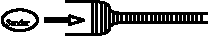
\includegraphics[scale=0.7]{chapters/failed/img/bottleneck_link}

\end{figure}

E' fisicamente impossibile per il delivery rate operare al di sopra del bottleneck rate. 

\section{Il sending rate e la congestione di rete}

%\begin{nota}{Nota}
%
%La definizione di congestione presentata in basso, è ricavata da uno scenario semplificato, in cui comunicano un solo mittente ed un solo destinatario. Per i nostri scopi è più che sufficiente. Tuttavia, la semplificazione aiuta il lettore a comprendere in modo rapido le basi e l'essenza della congestione. \bigskip
%
%Non sarà dunque difficile generalizzare anche alla classica situazione che avremo su Internet, dove sono presenti non solo più flussi concorrenti, ma anche bidirezionali. \bigskip
%
%\end{nota}

Dalla definizione del bottleneck rate (\textit{BtlBw}), discende subito la seguente affermazione:

\begin{center}
\label{sending_bottleneck_cons}
\textit{Un sending rate > bottleneck rate porta ad una crescita del bottleneck buffer, con conseguente aumento dei ritardi}
\end{center}

Per poter caratterizzare il ritardo end-to-end introduciamo un altro parametro caratteristico del path di rete, ovvero il Round-trip-propagation-delay (\textit{RTprop}). \bigskip

L'\textit{RTprop} costituisce il minimo ritardo di propagazione, o se si vuole il limite inferiore dell'RTT per una data comunicazione. \bigskip

Ora, il mittente dovrà attendere un RTT prima d'iniziare una seconda fase d'invio. Infatti ricordiamo che l'RTT per un dato pacchetto, è il tempo che intercorre tra la trasmissione e la ricezione del relativo ack. In una tale fase:

\begin{itemize}

\item Se il sending rate fosse minore o prossimo al bottleneck rate, il mittente introdurrebbe nella rete un amount inflight\footnote{Quantità di dati inviata dal sender, ma non ancora riscontrata}, tale da non contribuire alla crescita del bottleneck buffer. Per cui in tali condizioni l'RTT = \textit{RTprop}:

\end{itemize}

\begin{figure}[H]

\center
\caption{Delivery rate and round trip time vs inflight part 1}
\label{Delivery_rate_round_trip_time_part_1}
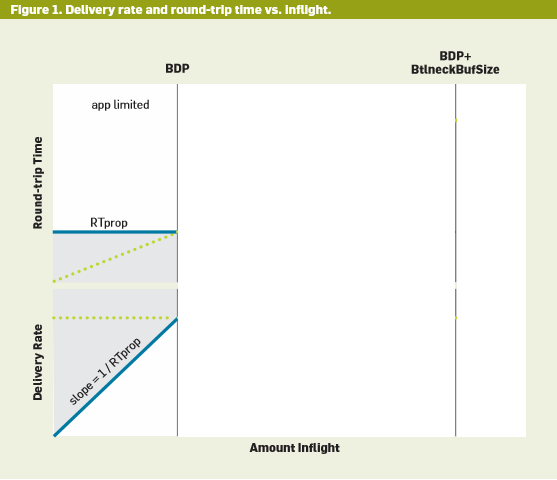
\includegraphics[scale=0.8]{chapters/failed/img/Delivery_rate_round_trip_time_part_1}
\caption*{Figura tratta da \cite[p.~60]{Cardwell:2017:BCC:3042068.3009824}}

\end{figure}

\begin{itemize}

\item Se il sending rate fosse superiore al bottleneck rate, il mittente introdurrebbe nella rete un amount inflight superiore alla capacità di quest'ultima. L'RTT aumenta, per via della crescita del bottleneck buffer, e per bilanciare l'amount inflight così da fissare il delivery rate sul bottleneck rate:

\end{itemize}

\begin{figure}[H]

\center
\caption{Delivery rate and round trip time vs inflight}
\label{Delivery_rate_round_trip_time}
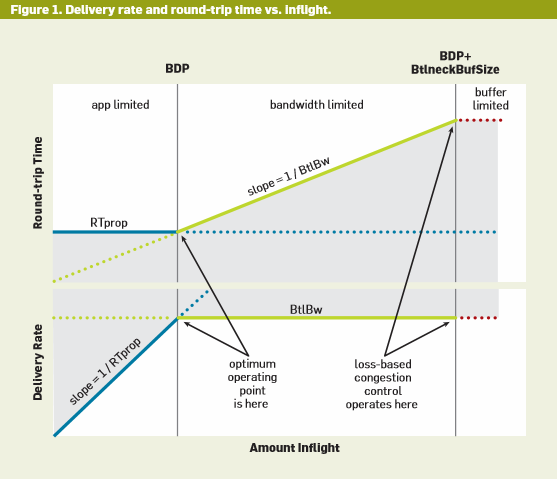
\includegraphics[scale=0.8]{chapters/failed/img/Delivery_rate_round_trip_time}
\caption*{Figura tratta da \cite[p.~60]{Cardwell:2017:BCC:3042068.3009824}}

\end{figure}

Questi due casi sono molto importanti, in quanto nel primo il mittente non contribuisce all'aumento dei ritardi, mentre nel secondo si. E' possibile quindi definire la condizione limite, che separa le due situazioni, introducendo il \textit{BDP} (bandwidth delay product \cite[p.~59]{Cardwell:2017:BCC:3042068.3009824}):

\[ BDP \:=\: BtlBw * RTprop \]

Esso definisce la capacità di rete, ovvero il massimo amount inflight che il mittente può introdurre nella rete in un \textit{RTprop}, al massimo delivery rate, senza contribuire nè alla generazione di code, nè all'espansione dei ritardi. \bigskip

\begin{suggerimento}{Osservazione: interpretazione fisica dei parametri caratteristici}

Per fornire una immagine più coincisa di tali parametri, possiamo immaginare una pipe virtuale tra il mittente ed il destinatario. Il \textit{BtlBw} definisce il diametro della pipe, l’\textit{RTprop} la sua lunghezza, mentre il \textit{BDP} la sua capacità (per definizione). \bigskip

\end{suggerimento}

Ora abbiamo tutti gli elementi per comprendere in che condizione il mittente contribuisce ad una congestione di rete, basta trasmettere in un \textit{RTprop} una quantità di dati superiore al \textit{BDP} corrente (pipe overfill). \bigskip

\section{Gli approcci loss based}

Tali approcci limitano il sending rate del mittente, ponendo un limite superiore per l'inflight amount: la congestion window (\texttt{cwnd}). \bigskip

Sulla base delle proprie informazioni locali, l'algoritmo modula la congestion window nel corso del tempo. \bigskip

La modulazione provvede semplicemente ad incrementare la \texttt{cwnd} (ogni versione usa tecniche differenti) , finchè non si verifica o un evento di timeout, o un evento di loss. \bigskip

Nel caso di un timeout, si porta la \texttt{cwnd} al valore minimo, in quanto si assume perso tutto ciò che è stato tramesso (anche il BBR manterrà questo comportamento).
Nel caso di un packet loss, la \texttt{cwnd} subisce un decremento moltiplicativo di un fattore $ \beta $. \bigskip

Quest'approccio non produce un controllo accurato del sending rate. Non è infatti possibile rilevare il momento in cui quest'ultimo eccede il bottleneck rate. \bigskip

Il risultato conseguente sono condizioni operative altalenanti, in cui per la maggior parte si espandono i ritardi, e caricano i buffer intermedi. \bigskip

Per essere più specifici, a seconda delle dimensioni dei buffer intermedi (in particolare del bottleneck buffer), potremmo riscontrare i seguenti problemi:

\begin{itemize}

\item \textit{Shallow buffers} : in virtù della loro piccola dimensione, saranno molto frequenti i fenomeni di perdita. Una strategia AIMD porta a decrementi multipli continui della congestion window, quindi un delivery rate di piccola entità;

\item \textit{Deep buffers} : l'algoritmo reagirà nel momento in cui il bottleneck buffer sarà completamente saturo. L'RTT avrà raggiunto in questa condizione il suo picco massimo: valore che cresce all'aumentare della BtlneckBufSize. 
Quindi nel corso del tempo, è favorita la progressione dei ritardi, e delle perdite.

\end{itemize}

In aggiunta le perdite portano a dedicare parte della banda alle ritrasmissioni. \bigskip

A questo punto è comprensibile la necessità di ricercare una strategia alternativa per limitare il sending rate, che non sia proibitiva in termini di loss rate, e che porti il delivery rate in prossimità del bottleneck rate.